\documentclass[11pt,a4paper]{article}
\usepackage[margin=2.3cm,headheight=14pt]{geometry}
\usepackage{lmodern}
\usepackage[T1]{fontenc}
\usepackage{amsmath,amssymb,bm}
\usepackage{booktabs,array,tabularx,multirow}
\usepackage{graphicx}
\usepackage[dvipsnames]{xcolor}
\usepackage{tikz}
\usetikzlibrary{arrows.meta,calc,patterns,decorations.pathreplacing}
\usepackage[skins,breakable]{tcolorbox}
\usepackage{caption,subcaption}
\usepackage{float}
\usepackage{fancyhdr}
\usepackage{enumitem}
\usepackage{siunitx}
\usepackage{microtype}
\usepackage[colorlinks=true,linkcolor=NavyBlue,citecolor=NavyBlue,urlcolor=NavyBlue]{hyperref}

\sisetup{per-mode=symbol,detect-all}
\captionsetup{font=small,labelfont=bf}
\setlength{\parskip}{0.45em}
\setlength{\parindent}{0pt}
\numberwithin{equation}{section}

\graphicspath{{../}}

\definecolor{corr}{HTML}{C0392B}
\definecolor{note}{HTML}{1F4E79}
\definecolor{keybg}{HTML}{F3F7FB}

\newtcolorbox{remark}[1][Remark]{enhanced,breakable,colback=note!4,colframe=note,
  boxrule=0pt,leftrule=3pt,arc=0pt,left=6pt,right=6pt,top=4pt,bottom=4pt,
  title={\textbf{#1}},coltitle=note,colbacktitle=note!4,
  attach title to upper={\ \ },fonttitle=\small}
\newtcolorbox{keyresult}{enhanced,colback=keybg,colframe=note!60,boxrule=0.6pt,arc=2pt,
  left=8pt,right=8pt,top=4pt,bottom=4pt}

\pagestyle{fancy}
\fancyhf{}
\fancyhead[L]{\small Eccentric-cavity soft bending actuator}
\fancyhead[R]{\small B.Tech Project: analytical derivation}
\fancyfoot[C]{\small\thepage}
\renewcommand{\headrulewidth}{0.4pt}

\newcommand{\Izz}{I_{zz}}
\newcommand{\rp}{r_p}
\newcommand{\tmin}{t_{\min}}
\newcommand{\tmax}{t_{\max}}

\begin{document}

%======================================================================
\begin{titlepage}
\centering
\vspace*{2.2cm}
{\large B.Tech Project\par}
\vspace{0.6cm}
{\LARGE\bfseries Pressure-to-Deflection Modelling of an\\[4pt]
Eccentric-Cavity Soft Pneumatic Bending Actuator\par}
\vspace{0.8cm}
{\large Analytical derivation and verification\\
by nonlinear finite-element analysis\par}
\vspace{1.6cm}

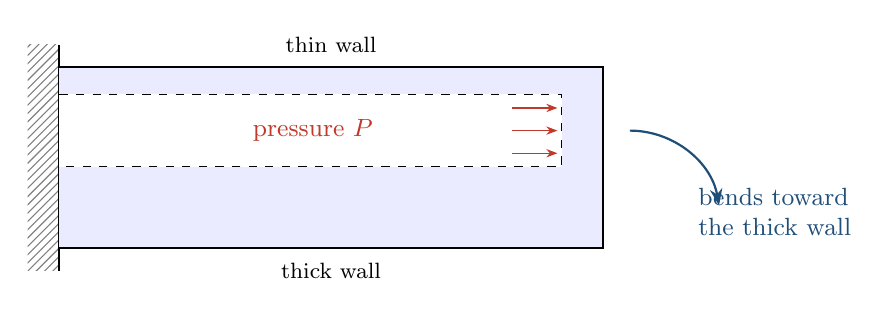
\begin{tikzpicture}[scale=1.15]
  % side view of the actuator, not to scale
  \fill[pattern=north east lines,pattern color=black!50] (-0.35,-1.25) rectangle (0,1.25);
  \draw[thick] (0,-1.25) -- (0,1.25);
  \fill[blue!8] (0,-1) rectangle (6,1);
  \draw[thick] (0,1) -- (6,1) -- (6,-1) -- (0,-1);
  \fill[white] (0,-0.1) rectangle (5.55,0.7);
  \draw[dashed] (0,0.7) -- (5.55,0.7) -- (5.55,-0.1) -- (0,-0.1);
  \foreach \y in {0.05,0.3,0.55} \draw[-{Stealth[length=4pt]},corr] (5.0,\y) -- (5.5,\y);
  \node[corr,font=\small] at (2.8,0.3) {pressure $P$};
  \draw[-{Stealth[length=6pt]},thick,note] (6.3,0.3) arc[start angle=90,end angle=10,radius=1.0];
  \node[note,font=\small,align=left] at (7.9,-0.6) {bends toward\\the thick wall};
  \node[font=\footnotesize] at (3,1.25) {thin wall};
  \node[font=\footnotesize] at (3,-1.25) {thick wall};
\end{tikzpicture}

\vspace{1.6cm}
{\large Rudranarayan Pradhan\par}
\vspace{0.3cm}
{\normalsize October 2026\par}
\vfill
\begin{minipage}{0.86\textwidth}
\small\textbf{Abstract.}
A silicone cylinder with an off-centre (eccentric) cavity bends when the cavity is pressurised.
This document derives the pressure-to-deflection relation of the actuator.
The cross-section properties, the eccentric thrust moment and the Euler--Bernoulli response are
derived step by step, and the validity of each result is stated.
Two physical results, both confirmed by a verified 3-D nonlinear finite-element (FE) model, decide how the beam result is used.
First, for a bare incompressible actuator the beam formula is multiplied by $(1-2\nu)$, which is zero for silicone.
Second, the bending a bare actuator does show is a finite-strain ballooning effect that is quadratic in $P$ at low pressure and ends at a limit pressure.
The beam formula is therefore the correct first-order model for a \emph{hoop-reinforced} actuator.
\end{minipage}
\vspace{0.8cm}
\end{titlepage}

\tableofcontents
\vspace{1em}
\begin{remark}[Units]
Units throughout: \si{mm}, \si{N}, \si{MPa} ($\SI{1}{MPa}=\SI{1000}{kPa}=\SI{1}{N/mm^2}$).
Boxed equations are the main results; blue boxes are remarks.
\end{remark}

\newpage
%======================================================================
\section{Introduction}

\subsection{The device}
The actuator is a solid silicone cylinder of outer radius $R$ and pressurised length $l$. A circular
cavity of radius $r$ runs along it, with its centre offset by $\rp$ from the axis of the cylinder.
One wall is therefore thin, $\tmin = R-\rp-r$, and the opposite wall is thick, $\tmax = R+\rp-r$.
The base is clamped, the far end is sealed by a solid cap, and the cavity is pressurised to a gauge pressure $P$.
The actuator curls toward the thick wall (Figure~\ref{fig:geometry}).

\textbf{Objective.} Find the map from the input $P$ to the tip bending angle $\theta$ and the tip deflection $\delta$.

\begin{figure}[H]
\centering
\begin{subfigure}[b]{0.52\textwidth}\centering
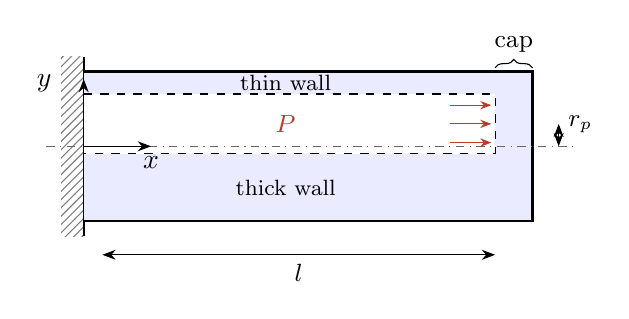
\begin{tikzpicture}[scale=0.95]
  \fill[pattern=north east lines,pattern color=black!50] (-0.3,-1.2) rectangle (0,1.2);
  \draw[thick] (0,-1.2) -- (0,1.2);
  \fill[blue!8] (0,-1) rectangle (6,1);
  \draw[thick] (0,1) -- (6,1) -- (6,-1) -- (0,-1);
  \fill[white] (0,-0.1) rectangle (5.5,0.7);
  \draw[dashed] (0,0.7) -- (5.5,0.7) -- (5.5,-0.1) -- (0,-0.1);
  \draw[dash dot,black!60] (-0.5,0) -- (6.6,0);
  \draw[-{Stealth}] (0,0) -- (0.9,0) node[below] {$x$};
  \draw[-{Stealth}] (0,0) -- (0,0.9);
  \node[left] at (-0.3,0.85) {$y$};
  \draw[{Stealth}-{Stealth}] (6.35,0) -- (6.35,0.3) node[right,font=\small] {$\rp$};
  \draw[{Stealth}-{Stealth}] (0.25,-1.45) -- (5.5,-1.45) node[midway,below,font=\small] {$l$};
  \draw[decorate,decoration={brace,amplitude=3pt}] (5.5,1.05) -- (6,1.05) node[midway,above=2pt,font=\small] {cap};
  \foreach \y in {0.05,0.3,0.55} \draw[-{Stealth[length=4pt]},corr] (4.9,\y) -- (5.45,\y);
  \node[corr,font=\small] at (2.7,0.3) {$P$};
  \node[font=\footnotesize] at (2.7,0.85) {thin wall};
  \node[font=\footnotesize] at (2.7,-0.55) {thick wall};
\end{tikzpicture}
\caption{Side view (bending plane $x$--$y$).}
\end{subfigure}\hfill
\begin{subfigure}[b]{0.44\textwidth}\centering
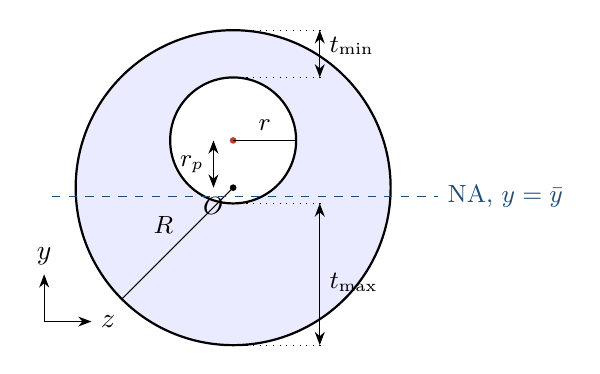
\begin{tikzpicture}[scale=1.0]
  \fill[blue!8] (0,0) circle (2);
  \draw[thick] (0,0) circle (2);
  \fill[white] (0,0.6) circle (0.8);
  \draw[thick] (0,0.6) circle (0.8);
  \draw[-{Stealth}] (-2.4,-1.7) -- (-1.8,-1.7) node[right] {$z$};
  \draw[-{Stealth}] (-2.4,-1.7) -- (-2.4,-1.1) node[above] {$y$};
  \fill (0,0) circle (1.2pt) node[below left,font=\small] {$O$};
  \fill[corr] (0,0.6) circle (1.2pt);
  \draw (0,0.6) -- (0.8,0.6) node[midway,above,font=\small] {$r$};
  \draw (0,0) -- (-1.414,-1.414) node[midway,above left,font=\small,xshift=2pt] {$R$};
  \draw[{Stealth}-{Stealth}] (-0.25,0) -- (-0.25,0.6) node[midway,left,font=\small] {$\rp$};
  \draw[dashed,note] (-2.3,-0.114) -- (2.6,-0.114) node[right,font=\small] {NA, $y=\bar y$};
  \draw[{Stealth}-{Stealth}] (1.1,1.4) -- (1.1,2.0);
  \node[right,font=\small] at (1.1,1.8) {$\tmin$};
  \draw[{Stealth}-{Stealth}] (1.1,-0.2) -- (1.1,-2.0);
  \node[right,font=\small] at (1.1,-1.2) {$\tmax$};
  \draw[dotted] (0,1.4) -- (1.15,1.4); \draw[dotted] (0,-0.2) -- (1.15,-0.2);
  \draw[dotted] (0,2.0) -- (1.15,2.0); \draw[dotted] (0,-2.0) -- (1.15,-2.0);
\end{tikzpicture}
\caption{Cross-section.}
\end{subfigure}
\caption{Geometry and coordinate frame. The origin $O$ is the centre of the outer circle, the cavity centre
is at $(y,z)=(\rp,0)$ and the neutral axis (NA) lies at $y=\bar y<0$. Not to scale.}
\label{fig:geometry}
\end{figure}

\subsection{Scope}
Sections~\ref{sec:section}--\ref{sec:beam} derive the cross-section properties, the pressure loading and the
beam response. Section~\ref{sec:poisson} adds the effect of the in-plane wall stresses, which decides whether
a bare actuator bends at first order. Section~\ref{sec:wall} analyses the asymmetric expansion of the
thin and thick walls. Section~\ref{sec:tiers} lists the model hierarchy and
Section~\ref{sec:fea} summarises the FE verification. All numerical values refer to the
\emph{placeholder} design $R=10$, $r=4$, $\rp=3$, $l=\SI{100}{mm}$ with a neo-Hookean silicone of $E=\SI{0.6}{MPa}$.

%======================================================================
\section{Notation and assumptions}

\begin{table}[H]
\centering\small
\begin{tabular}{@{}lll@{}}
\toprule
Symbol & Meaning & Placeholder value \\
\midrule
$R$ & outer radius & \SI{10}{mm}\\
$r$ & cavity radius & \SI{4}{mm}\\
$\rp$ & cavity eccentricity (offset of the cavity centre along $+y$) & \SI{3}{mm}\\
$l$ & pressurised length & \SI{100}{mm}\\
$\tmin,\ \tmax$ & thinnest and thickest wall, $R\mp\rp-r$ & \SI{3}{mm}, \SI{9}{mm}\\
$E,\ \mu,\ \nu$ & small-strain Young's modulus, shear modulus, Poisson's ratio & \SI{0.6}{MPa}, \SI{0.2}{MPa}, $\approx 0.5$\\
$C_{10},C_{20},C_{30}$ & Yeoh coefficients (neo-Hookean: $C_{10}=\mu/2=E/6$ only) & $C_{10}=\SI{0.1}{MPa}$\\
$P$ & gauge pressure in the cavity (the input) & \SIrange{0}{110}{kPa}\\
$A,\ A_c$ & elastomer area, cavity area $\pi r^2$ & \\
$\bar y,\ \Izz,\ e$ & neutral-axis position, second moment about it, moment arm & \\
$\kappa,\ \theta,\ \delta$ & curvature, tip angle, tip deflection & \\
\bottomrule
\end{tabular}
\caption{Symbols. Axes: $x$ along the actuator (base at $x=0$, tip at $x=l$); $y$ in the section, from the
outer centre toward the cavity centre; $z$ completes the right-handed frame. Bending is about $z$, toward $-y$.}
\end{table}

\textbf{Assumptions.}
\begin{enumerate}[nosep,label=(A\arabic*)]
\item The material is isotropic, homogeneous, rate-independent and (nearly) incompressible; Mullins and
viscoelastic effects are removed by preconditioning.
\item The pressure is uniform in the cavity; gravity and external loads are neglected; the base is clamped and the tip is free.
\item \emph{Beam model only:} plane sections remain plane, the cross-section keeps its shape, and every longitudinal
fibre is in uniaxial stress. Assumption (A3) holds for a hoop-reinforced actuator and fails for a bare one (Section~\ref{sec:poisson}).
\end{enumerate}

%======================================================================
\section{Cross-section geometry}\label{sec:section}

\subsection{Elastomer area}
The section is the outer disc minus the cavity disc:
\begin{equation}
A = \pi R^2 - \pi r^2 = \pi\,(R^2-r^2). \label{eq:A}
\end{equation}

\subsection{Neutral axis}
Treat the cavity as a negative area centred at $y=\rp$. The centroid of the composite area is
\begin{equation}
\bar y = \frac{\pi R^2\cdot 0 \;-\; \pi r^2\cdot \rp}{\pi R^2-\pi r^2}
\quad\Longrightarrow\quad
\boxed{\;\bar y = -\,\frac{r^2\,\rp}{R^2-r^2}\;} \label{eq:ybar}
\end{equation}
The neutral axis sits on the thick-wall side of the outer centre ($\bar y<0$), because material has been removed on the $+y$ side.
Dimensional check: $r^2\rp/(R^2-r^2)$ is a length.

\subsection{Second moment of area about the neutral axis}
By the parallel-axis theorem $I = I_c + A d^2$ applied to each disc, with distances measured from the neutral axis:
\begin{equation}
\Izz = \Big[\frac{\pi R^4}{4} + \pi R^2\,\bar y^{\,2}\Big] - \Big[\frac{\pi r^4}{4} + \pi r^2\,(\rp-\bar y)^2\Big].
\end{equation}
To simplify, note that $\rp - \bar y = \rp + \dfrac{r^2\rp}{R^2-r^2} = \dfrac{R^2\rp}{R^2-r^2}$. Then
\begin{align}
\pi R^2\bar y^{\,2} - \pi r^2(\rp-\bar y)^2
&= \frac{\pi\,\rp^2}{(R^2-r^2)^2}\Big[R^2 r^4 - r^2 R^4\Big]
 = -\,\frac{\pi R^2 r^2 \rp^2\,(R^2-r^2)}{(R^2-r^2)^2}
 = -\,\frac{\pi R^2 r^2 \rp^2}{R^2-r^2},
\end{align}
so
\begin{equation}
\boxed{\;\Izz = \frac{\pi\,(R^4-r^4)}{4} - \frac{\pi R^2 r^2 \rp^2}{R^2-r^2}\;} \label{eq:I}
\end{equation}
The first term is the concentric hollow cylinder; the second is the stiffness lost by shifting the hole off-centre.
For the placeholder design $\Izz = \pi(2436 - 171.43) = \SI{7114.4}{mm^4}$
(the parallel-axis form evaluated numerically gives the same value).

%======================================================================
\section{Pressure loading}\label{sec:load}

\subsection{Thrust on the sealed tip}
The pressure acts on the inside face of the tip cap, whose projected area is the cavity area $A_c = \pi r^2$:
\begin{equation}
F = P\,A_c = P\,\pi r^2 . \label{eq:F}
\end{equation}

Note that the thrust uses the cavity area $A_c$, not the elastomer area $A$ of eq.~(\ref{eq:A}).

\subsection{Moment arm}
The resultant of a uniform pressure on a circular face passes through the centre of the circle, $y=\rp$.
Its distance from the neutral axis is
\begin{equation}
e = \rp - \bar y = \rp + \frac{r^2\rp}{R^2-r^2}
\quad\Longrightarrow\quad
\boxed{\;e = \frac{R^2\,\rp}{R^2-r^2}\;} \label{eq:e}
\end{equation}

\subsection{Bending moment}
\begin{equation}
\boxed{\;M = F\,e = \frac{\pi P R^2 r^2 \rp}{R^2-r^2}\;} \label{eq:M}
\end{equation}

\begin{figure}[H]
\centering
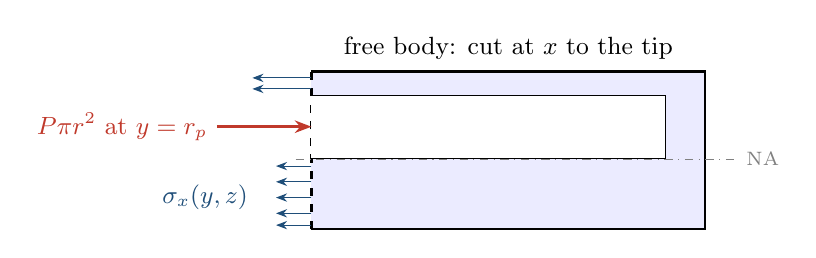
\begin{tikzpicture}[scale=1.0]
  \fill[blue!8] (0,-1) rectangle (5,1);
  \draw[thick] (0,1) -- (5,1) -- (5,-1) -- (0,-1);
  \draw[thick,dashed] (0,-1) -- (0,1);
  \fill[white] (0,-0.1) rectangle (4.5,0.7);
  \draw (0,0.7) -- (4.5,0.7) -- (4.5,-0.1) -- (0,-0.1);
  \node[font=\small] at (2.5,1.3) {free body: cut at $x$ to the tip};
  % fluid force at the cut
  \draw[-{Stealth[length=6pt]},very thick,corr] (-1.2,0.3) -- (0,0.3);
  \node[corr,left,font=\small] at (-1.2,0.3) {$P\pi r^2$ at $y=\rp$};
  % silicone stress at the cut
  \foreach \y in {0.78,0.92} \draw[-{Stealth[length=4pt]},note] (0,\y) -- (-0.75,\y);
  \foreach \y in {-0.2,-0.4,-0.6,-0.8,-0.95} \draw[-{Stealth[length=4pt]},note] (0,\y) -- (-0.45,\y);
  \node[note,font=\small] at (-1.35,-0.6) {$\sigma_x(y,z)$};
  \draw[dash dot,black!50] (-0.2,-0.114) -- (5.4,-0.114) node[right,font=\scriptsize] {NA};
\end{tikzpicture}
\caption{Free body from a cut at $x$ to the tip, silicone together with the fluid it encloses. The fluid beyond the cut
pushes with $P\pi r^2$ through the cavity centre; the silicone carries the axial stress $\sigma_x$.}
\label{fig:fbd}
\end{figure}

\begin{remark}[Why $M$ is uniform along the length]
Cut the actuator at any $x$ and take the free body from the cut to the tip, \emph{including the fluid inside it}
(Figure~\ref{fig:fbd}). No external force acts on it except at the cut. Equilibrium gives
\begin{equation}
\int_A \sigma_x\,dA = P\pi r^2 ,\qquad \int_A \sigma_x\,(y-\rp)\,dA = 0 . \label{eq:fbd}
\end{equation}
So the wall is in net tension $N=P\pi r^2$ and the stress resultant acts through the cavity centre. About the neutral axis this
is the moment $M = N e$ of eq.~(\ref{eq:M}), at every $x$ and for any material law.
Eq.~(\ref{eq:fbd}) fixes the \emph{resultants} of $\sigma_x$ only; turning them into strain needs a constitutive assumption (Sections~\ref{sec:beam} and~\ref{sec:poisson}).
\end{remark}

%======================================================================
\section{Beam-theory response (Euler--Bernoulli)}\label{sec:beam}

Under assumption (A3), $\sigma_x = E\,\varepsilon_x$ with $\varepsilon_x = \varepsilon_0 + \kappa\,(y-\bar y)$.

\subsection{Curvature}
\begin{equation}
\boxed{\;\kappa = \frac{1}{\rho} = \frac{M}{E\Izz} = \frac{\pi P R^2 r^2 \rp}{E\,\Izz\,(R^2-r^2)}\;} \label{eq:kappa}
\end{equation}

Here $E$ is the small-strain modulus, $E = 3\mu = 6C_{10}$ for an incompressible solid. A secant modulus chosen to
fit a curve would hide the real nonlinearity, which for the bare actuator is ballooning (Section~\ref{sec:wall}), not a softening of $E$.

\subsection{Tip bending angle}
$M$ is uniform, so $\kappa$ is uniform and the centreline is a circular arc:
\begin{equation}
\boxed{\;\theta = \kappa\,l = \frac{M\,l}{E\Izz} = \frac{\pi P R^2 r^2 \rp\, l}{E\,\Izz\,(R^2-r^2)}\;} \label{eq:theta}
\end{equation}

The tip angle is linear in $P$, since $\kappa$ is.

\subsection{Tip deflection}
For an arc of radius $\rho=1/\kappa$ turning through $\theta$, the tip moves sideways by
\begin{equation}
\delta = \rho\,(1-\cos\theta) = \frac{1-\cos\theta}{\kappa} = \frac{l}{\theta}\,(1-\cos\theta). \label{eq:delta-arc}
\end{equation}
For $\theta\ll 1$, $1-\cos\theta \approx \theta^2/2$ and
\begin{equation}
\delta \approx \frac{\theta\, l}{2} = \frac{M\,l^2}{2E\Izz}, \label{eq:delta-small}
\end{equation}
which is the cantilever result for a uniform end moment.
The axial tip position is $x_{\text{tip}} = \rho\sin\theta$.

\subsection{Axial elongation}
The net tension of eq.~(\ref{eq:fbd}) stretches the centroidal fibre by $\varepsilon_0 = F/(EA)$, so $\Delta l = Fl/(EA)$.
A uniform axial strain moves every fibre by the same amount and does not shift the neutral axis.
This elongation holds under assumption (A3), i.e.\ for a hoop-reinforced actuator; for a bare incompressible actuator the first-order
elongation is $(1-2\nu)Fl/(EA)\approx 0$ (Section~\ref{sec:poisson}).

\subsection{Non-dimensional form}
Writing $\hat I = \Izz/R^4$,
\begin{equation}
\theta = \frac{P}{E}\,\frac{l}{R}\; f\!\left(\frac{r}{R},\frac{\rp}{R}\right),\qquad
f = \frac{\pi\,(r/R)^2\,(\rp/R)}{\hat I\,\big(1-(r/R)^2\big)} .
\end{equation}
The response is linear in $P/E$ and in the slenderness $l/R$. The section shape enters only through $f$.
For the placeholder design $\hat I = 0.7114$ and $f = 0.2523$.

\subsection{Worked example}
\begin{table}[H]
\centering\small
\begin{tabular}{@{}lr@{\qquad}lr@{}}
\toprule
\multicolumn{2}{c}{Section (eqs.~\ref{eq:A}--\ref{eq:e})} & \multicolumn{2}{c}{Response at $P=\SI{20}{kPa}$ (eqs.~\ref{eq:F}--\ref{eq:delta-small})}\\
\midrule
$A$ & \SI{263.9}{mm^2} & $F$ & \SI{1.005}{N}\\
$\bar y$ & \SI{-0.571}{mm} & $M$ & \SI{3.590}{N\,mm}\\
$\Izz$ & \SI{7114.4}{mm^4} & $\kappa$ & \SI{8.41e-4}{mm^{-1}}\\
$e$ & \SI{3.571}{mm} & $\theta$ & \SI{4.82}{\degree}\\
$\tmin,\ \tmax$ & \SI{3}{mm}, \SI{9}{mm} & $\delta$ arc / small-angle & \SI{4.203}{mm} / \SI{4.206}{mm}\\
\bottomrule
\end{tabular}
\caption{Beam model for the placeholder design, $E=\SI{0.6}{MPa}$. At \SIlist{10;40;60}{kPa}: $\theta = \SIlist{2.41;9.64;14.46}{\degree}$, $\delta_{\text{arc}} = \SIlist{2.10;8.39;12.55}{mm}$.}
\label{tab:example}
\end{table}

\begin{keyresult}
\textbf{Validity of eqs.~(\ref{eq:kappa})--(\ref{eq:delta-small}).} They rest on assumption (A3): each fibre carries only axial stress.
That is true when a hoop-fibre sleeve (thread wrap) carries the hoop load. The FE model confirms that for the \emph{sleeved} actuator the tip angle matches
eq.~(\ref{eq:theta}) within 5\,\% up to $P/E\approx 0.03$. For the \emph{bare} actuator see the next section.
\end{keyresult}

%======================================================================
\section{The bare actuator: effect of the in-plane wall stresses}\label{sec:poisson}

The pressure does not only push on the tip cap. It also loads the wall \emph{in the plane of the section}: radial compression
at the cavity surface and hoop tension around it, both of order $P$ or larger. Assumption (A3) ignores them.
In linear isotropic elasticity they enter the axial strain through Poisson's ratio:
\begin{equation}
\varepsilon_x = \frac{\sigma_x - \nu(\sigma_y+\sigma_z)}{E}
\quad\Longrightarrow\quad
\sigma_x = E\big[\varepsilon_0 + \kappa(y-\bar y)\big] + \nu\,(\sigma_y+\sigma_z). \label{eq:hooke}
\end{equation}

\subsection{Resultants of the in-plane stresses}
The in-plane field need not be solved: its resultant and first moment follow from equilibrium alone.
Far from the ends the in-plane stresses $\sigma_{\alpha\beta}$ ($\alpha,\beta\in\{y,z\}$) satisfy $\partial_\beta\sigma_{\alpha\beta}=0$, the outer surface is traction-free and the cavity surface
carries the traction $P\,\bm m$, where $\bm m$ is the unit normal pointing out of the cavity into the wall. Take coordinates $\bm x'$ centred on the cavity. From the identities
\[
\partial_\beta(\sigma_{\alpha\beta}x'_\alpha) = \sigma_{\alpha\alpha},\qquad
\partial_\beta(\sigma_{\alpha\beta}x'_\alpha x'_\gamma) - \partial_\beta\!\big(\sigma_{\gamma\beta}\,\tfrac12|\bm x'|^2\big) = \sigma_{\alpha\alpha}\,x'_\gamma
\]
and the divergence theorem, with $\bm x' = r\bm m$ on the cavity boundary,
\begin{equation}
\int_A(\sigma_y+\sigma_z)\,dA = \oint P\,r\,ds = 2P\pi r^2,\qquad
\int_A(\sigma_y+\sigma_z)\,x'_\gamma\,dA = \oint P\,r^2 m_\gamma\,ds - \oint \tfrac{P r^2}{2}\, m_\gamma\,ds = 0 .
\end{equation}
So the in-plane stresses have a total of $2P\pi r^2$ acting \emph{through the cavity centre}, for an outer boundary of any shape.
About the neutral axis:
\begin{equation}
\int_A(\sigma_y+\sigma_z)\,dA = 2P\pi r^2,\qquad \int_A(\sigma_y+\sigma_z)(y-\bar y)\,dA = 2P\pi r^2\,e .
\end{equation}

\subsection{Corrected first-order response}
Substitute eq.~(\ref{eq:hooke}) into the two free-body conditions (\ref{eq:fbd}), using $\int_A (y-\bar y)\,dA = 0$:
\begin{align}
\text{force:}\quad & EA\,\varepsilon_0 + 2\nu P\pi r^2 = P\pi r^2,\\
\text{moment:}\quad & E\Izz\,\kappa + 2\nu P\pi r^2 e = P\pi r^2 e .
\end{align}
\begin{keyresult}
\begin{equation}
\varepsilon_0 = (1-2\nu)\,\frac{P\pi r^2}{EA},\qquad
\kappa = (1-2\nu)\,\frac{M}{E\Izz} = (1-2\nu)\,\frac{\pi P R^2 r^2 \rp}{E\,\Izz\,(R^2-r^2)} . \label{eq:poisson}
\end{equation}
For silicone $\nu\to 0.5$: \textbf{in the small-strain limit a bare eccentric-cavity actuator neither lengthens nor bends.}
\end{keyresult}

The first result is the textbook statement that a closed incompressible tube does not lengthen under internal pressure;
the second is its bending counterpart. The thrust moment is still there, but the Poisson effect of the in-plane stresses cancels it exactly.
The beam results of Section~\ref{sec:beam} therefore apply to the hoop-reinforced actuator, and eq.~(\ref{eq:poisson}) to the bare one.

\begin{remark}[FE check of eq.~(\ref{eq:poisson})]
Mid-span curvature from the FE model divided by eq.~(\ref{eq:kappa}), at $P/E=10^{-5}$:
\begin{center}\small
\begin{tabular}{@{}lcccccc@{}}
\toprule
$\nu$ & 0 & 0.2 & 0.3 & 0.4 & 0.45 & 0.4995\\
\midrule
FE & 1.0000 & 0.6001 & 0.4001 & 0.2002 & 0.1002 & 0.0012\\
$1-2\nu$ & 1.0000 & 0.6000 & 0.4000 & 0.2000 & 0.1000 & 0.0010\\
\bottomrule
\end{tabular}
\end{center}
The tip angle of the nearly incompressible actuator is not exactly zero but 6\,\% of eq.~(\ref{eq:theta}). All of it comes from the two ends,
where the clamp and the cap stop the wall from expanding and switch the cancellation off locally.
\end{remark}

%======================================================================
\section{Asymmetric wall expansion}\label{sec:wall}

There is a second bending mechanism. The thin wall stretches more in hoop than the thick wall, the
stretch couples into axial lengthening, and the thin side becomes longer than the thick side. This section derives the wall
geometry, shows why a linear estimate of this effect fails, and gives the correct finite-strain result.

\subsection{Wall thickness around the cavity}
\begin{figure}[H]
\centering
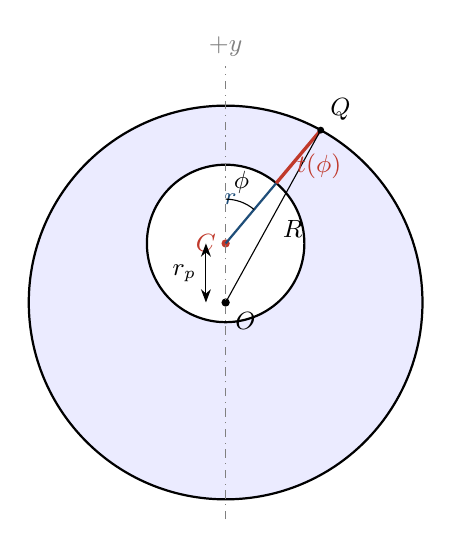
\begin{tikzpicture}[scale=1.25]
  \fill[blue!8] (0,0) circle (2);
  \draw[thick] (0,0) circle (2);
  \fill[white] (0,0.6) circle (0.8);
  \draw[thick] (0,0.6) circle (0.8);
  \fill (0,0) circle (1.2pt) node[below right,font=\small] {$O$};
  \fill[corr] (0,0.6) circle (1.2pt) node[left,font=\small] {$C$};
  \draw[dash dot,black!50] (0,-2.2) -- (0,2.4) node[above,font=\small] {$+y$};
  \draw[thick,note] (0,0.6) -- (0.5142,1.2128);
  \draw[very thick,corr] (0.5142,1.2128) -- (0.9661,1.7513);
  \draw (0,0) -- (0.9661,1.7513);
  \node[note,font=\small] at (0.05,1.05) {$r$};
  \node[corr,font=\small] at (0.95,1.38) {$t(\phi)$};
  \node[font=\small] at (0.68,0.75) {$R$};
  \draw (0,1.05) arc[start angle=90,end angle=50,radius=0.45];
  \node[font=\small] at (0.16,1.22) {$\phi$};
  \fill (0.9661,1.7513) circle (1pt) node[above right,font=\small] {$Q$};
  \draw[{Stealth}-{Stealth}] (-0.2,0) -- (-0.2,0.6) node[midway,left,font=\small] {$\rp$};
\end{tikzpicture}
\caption{Wall thickness along a ray from the cavity centre $C$ at angle $\phi$ from $+y$. $\phi=0$ points at the thin wall.}
\label{fig:tphi}
\end{figure}
Along a ray from the cavity centre $C$ at angle $\phi$ from $+y$ (Figure~\ref{fig:tphi}), the point $Q$ at distance $s=r+t$ lies on the outer circle.
The law of cosines in triangle $OCQ$ gives
\begin{equation}
R^2 = \rp^2 + s^2 + 2\rp s\cos\phi
\quad\Longrightarrow\quad
s = -\rp\cos\phi + \sqrt{R^2-\rp^2\sin^2\phi},
\end{equation}
taking the positive root, so
\begin{equation}
\boxed{\;t(\phi) = \sqrt{R^2-\rp^2\sin^2\phi} \;-\; \rp\cos\phi \;-\; r\;} \label{eq:tphi}
\end{equation}
with $t(0) = R-\rp-r = \tmin$ and $t(\pi) = R+\rp-r = \tmax$. The expression is exact for the radial wall thickness along the ray.
The FE mesh is built on this formula. As before, the longitudinal strain and stress are $\varepsilon_x$ and $\sigma_x$, since the actuator axis is $x$.

\subsection{Hoop stress}
In the thin-membrane approximation the hoop stress at angle $\phi$ is $\sigma_\theta(\phi)\approx P r/t(\phi)$, and the mean axial stress is
$\bar\sigma_x = P\pi r^2/A$. The membrane estimate needs $t\ll r$; here $\tmin/r = 0.75$, so the values are indicative only.

\subsection{A linear estimate, and why it fails}
A first guess takes $\varepsilon_x(\phi)\propto Pr/(E\,t(\phi))$ and defines
\begin{equation}
\kappa_{\exp} \approx \frac{\varepsilon_x(\text{thin})-\varepsilon_x(\text{thick})}{2R} = \frac{P r}{2ER}\left(\frac{1}{R-\rp-r}-\frac{1}{R+\rp-r}\right), \label{eq:kexp}
\end{equation}
to be added to the thrust curvature, $\kappa_{\text{total}}=\kappa_{\text{thrust}}+\kappa_{\exp}$. This estimate does not hold:
\begin{enumerate}[nosep]
\item It rests on linear Poisson coupling, and Section~\ref{sec:poisson} shows that for $\nu=0.5$ linear elasticity gives \emph{no} axial strain and \emph{no} curvature from pressure at all.
The linear in-plane effect is exactly what cancels $\kappa_{\text{thrust}}$; it cannot also add to it.
\item The superposition $\kappa_{\text{total}}=\kappa_{\text{thrust}}+\kappa_{\exp}$ is linear in $P$ and equals $2.76\,\kappa_{\text{thrust}}$ at every pressure for the placeholder design.
The FE curvature of the bare actuator runs from $0.1$ to $3$ times $\kappa_{\text{thrust}}$ over the pressure range: it is not linear in $P$.
\end{enumerate}

\subsection{The correct mechanism: second-order lengthening}
Consider a thin closed neo-Hookean tube with hoop, axial and thickness stretches $\lambda_1=1+a$, $\lambda_2=1+b$, $\lambda_3=1/(\lambda_1\lambda_2)$.
The membrane stresses are $\sigma_\theta=\mu(\lambda_1^2-\lambda_3^2)$ and $\sigma_x=\mu(\lambda_2^2-\lambda_3^2)$, and a closed end gives $\sigma_x=\sigma_\theta/2$:
\begin{equation}
2\lambda_2^2 = \lambda_1^2 + \lambda_3^2 .
\end{equation}
Expanding with $\lambda_3^2 \approx 1-2a-2b+3a^2+3b^2+4ab$:
\begin{itemize}[nosep]
\item first order: $4b = -2b$, so $b=0$. There is no axial strain at first order, in agreement with eq.~(\ref{eq:poisson});
\item second order, with $b=O(a^2)$: $6b = 4a^2$, so
\end{itemize}
\begin{equation}
\boxed{\;\varepsilon_{\text{axial}} \approx \tfrac{2}{3}\,\varepsilon_{\text{hoop}}^{\,2}\;} \label{eq:twothirds}
\end{equation}
The thin wall has the larger hoop strain, so it lengthens more and the actuator bends toward the thick wall. The
wall-expansion mechanism is therefore real, but it is \emph{quadratic} in $P$, not linear.

\begin{remark}[Scaling estimate]
Take the closed-tube membrane hoop strain $\varepsilon_{\text{hoop}} = \tfrac{3}{4}\,P r/(E\,t)$ for each wall, apply eq.~(\ref{eq:twothirds}), and divide the difference in axial strain by the distance between
the wall mid-lines ($d = \SI{14}{mm}$):
\[
\kappa_{\text{wall}} \approx \frac{2}{3}\,\frac{\varepsilon_{\text{hoop}}(\tmin)^2-\varepsilon_{\text{hoop}}(\tmax)^2}{d}.
\]
This gives $\SI{1.2e-5}{mm^{-1}}$ at \SI{10}{kPa} and $\SI{4.7e-5}{mm^{-1}}$ at \SI{20}{kPa}, against FE mid-span values of
$\num{1.8e-5}$ and $\SI{7.8e-5}{mm^{-1}}$. The estimate is within a factor of two and reproduces the $P^2$ scaling: the FE curvature grows by 4.3 when $P$ doubles.
It is a rough guide only, since the wall is not thin and the two walls interact.
\end{remark}

\subsection{Ballooning limit}
A rubber tube under internal pressure has a pressure maximum: past it, the wall thins faster than the hoop stress can rise, and the tube inflates without bound at falling pressure.
The thin wall reaches it first. For the placeholder shape the FE model gives the limit at
\begin{equation}
P_{\text{lim}} = 0.523\,\mu \quad(\SI{104.7}{kPa}\ \text{for}\ E=\SI{0.6}{MPa};\ \SI{14}{kPa}\ \text{for}\ E=\SI{0.08}{MPa}).
\end{equation}
Above $P_{\text{lim}}$ a neo-Hookean actuator has no equilibrium under pressure control. Under volume control (a water-filled syringe) the path through the limit is stable.
A real silicone stiffens at large stretch (Yeoh $C_{20},C_{30}>0$), which can raise or remove the limit, so the material must be measured before this number is trusted.
In short, wall compliance dominates the bare actuator: it is the only bending mechanism that survives, and it ends in a limit pressure.

%======================================================================
\section{Model hierarchy}\label{sec:tiers}

\begin{table}[H]
\centering\small
\begin{tabularx}{\textwidth}{@{}l>{\raggedright\arraybackslash}X>{\raggedright\arraybackslash}X@{}}
\toprule
Tier & Content & Applies to\\
\midrule
1 & Linear Euler--Bernoulli, eqs.~(\ref{eq:kappa})--(\ref{eq:delta-small}) & hoop-reinforced, $P/E\lesssim 0.03$\\
2 & Tier~1 curvature with large-rotation arc kinematics and axial stretch: $l_c = l(1+\varepsilon_0)$, $\rho = l_c/\theta$, $x_{\text{tip}} = \rho\sin\theta$, $\delta=\rho(1-\cos\theta)$ & hoop-reinforced; the form needed for control\\
3 & Hyperelastic section equilibrium: $\lambda(y) = \lambda_c + k(y-\rp)$; solve $\int s(\lambda)\,dA = P\pi r^2$, $\int s(\lambda)(y-\rp)\,dA=0$ with $s(\lambda) = 2(\lambda-\lambda^{-2})[C_{10}+2C_{20}(I_1-3)+3C_{30}(I_1-3)^2]$, $I_1=\lambda^2+2/\lambda$; then $\theta = kl$ & hoop-reinforced, larger $P$\\
4 & Nonlinear 3-D finite elements (Section~\ref{sec:fea}) & bare and reinforced, up to the limit point\\
5 & Experiment & material constants and validation\\
\bottomrule
\end{tabularx}
\caption{Model tiers. Tiers 1--3 share assumption (A3) and describe the hoop-reinforced actuator; the bare actuator needs Tier 4.}
\end{table}

%======================================================================
\section{Verification by nonlinear finite-element analysis}\label{sec:fea}

\subsection{What was done and how}
No commercial structural FE package was available, so a solver was written in Python with NumPy, SciPy and JAX (\texttt{actuator\_fea.py}):
\begin{itemize}[nosep]
\item \textbf{Mesh:} 27-node hexahedra, half model with symmetry about the bending plane (Figure~\ref{fig:mesh}); 588 elements (medium mesh); clamped base, solid tip cap of thickness $R/2$.
\item \textbf{Material:} Yeoh/neo-Hookean with an isochoric--volumetric split, mixed displacement--pressure (Q2/P1) formulation to avoid volumetric locking, $\nu = 0.4995$.
\item \textbf{Load:} follower pressure on every wetted cavity face, derived from the potential $-PV$ of the enclosed cavity volume.
\item \textbf{Solver:} Newton iteration with tangents from automatic differentiation; pressure control, switching automatically to volume control when a pressure step has no solution, so the limit point is passed and located.
\item \textbf{Variants:} bare actuator, and the same actuator with an ideal inextensible hoop-fibre sleeve on the outer surface.
\end{itemize}

\begin{figure}[H]
\centering
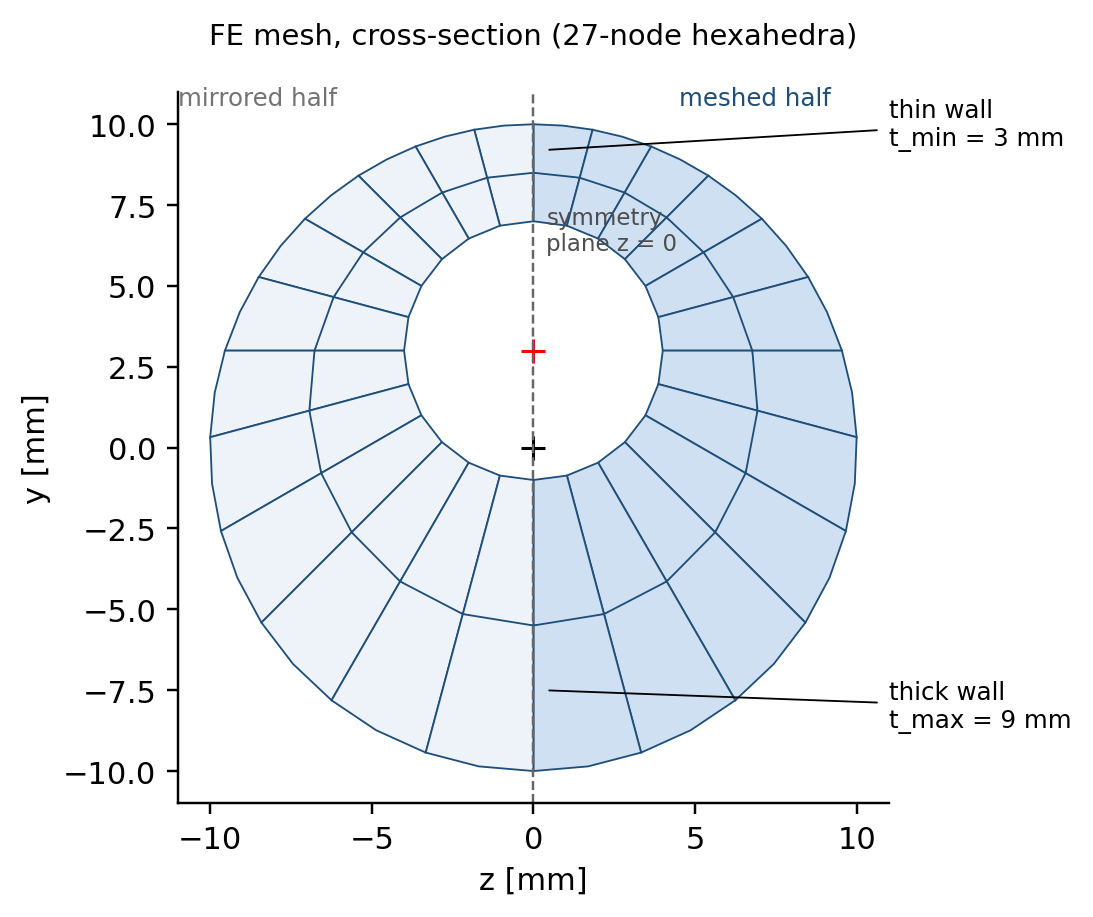
\includegraphics[width=0.48\textwidth]{figures/fe_mesh_section.png}
\caption{FE mesh of the cross-section. Only the half $z\ge0$ is solved; the other half follows by symmetry.}
\label{fig:mesh}
\end{figure}

\subsection{Verification of the solver}
\begin{table}[H]
\centering\small
\begin{tabularx}{\textwidth}{@{}>{\raggedright\arraybackslash}X>{\raggedright\arraybackslash}X>{\raggedright\arraybackslash}X@{}}
\toprule
Test & Reference & Largest deviation\\
\midrule
Uniaxial tension, $\lambda\le 3$ & exact incompressible stress & 0.2\,\% neo-Hookean; 2.5\,\% Yeoh at $\lambda=3$\\
Thick-walled tube inflation, $P/\mu\le0.7$ & exact neo-Hookean solution & 0.05\,\%\\
Small-pressure bending, $0\le\nu\le0.4995$ & $\kappa=(1-2\nu)M/(E\Izz)$ & 0.0002 (in units of eq.~\ref{eq:kappa})\\
Mesh refinement, $\delta$ at $P/\mu=0.30,\ 0.45$ & fine mesh, 1664 elements & medium mesh within 0.5\,\%\\
\bottomrule
\end{tabularx}
\caption{Verification (\texttt{fea\_verify.py}, log in \texttt{results/verification.log}).}
\end{table}

\subsection{Findings}
\begin{figure}[H]
\centering
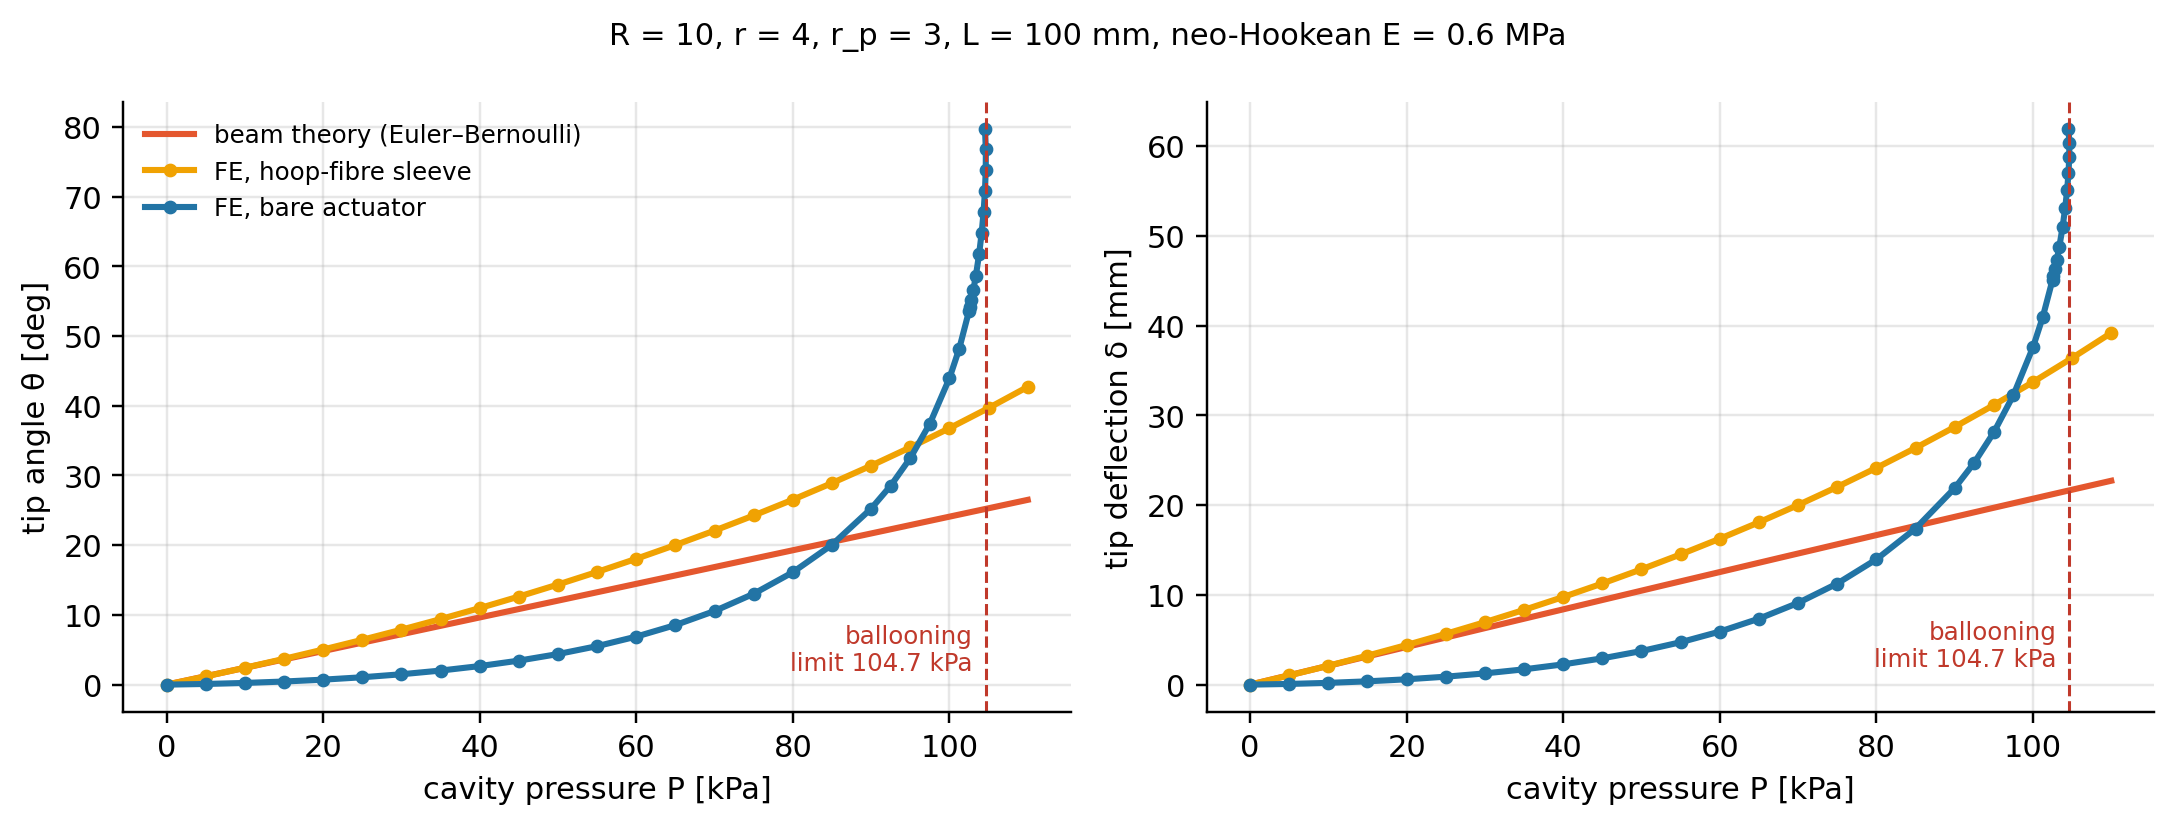
\includegraphics[width=\textwidth]{figures/fe_response.png}
\caption{Tip angle and tip deflection against pressure: beam theory (eq.~\ref{eq:theta}, \ref{eq:delta-arc}) and FE for the bare and the sleeved actuator.}
\label{fig:response}
\end{figure}

\begin{table}[H]
\centering\small
\begin{tabular}{@{}rccccc@{\qquad}cccc@{}}
\toprule
& & \multicolumn{4}{c}{Bare} & \multicolumn{4}{c}{Hoop-reinforced}\\
\cmidrule(lr){3-6}\cmidrule(lr){7-10}
$P$ [kPa] & $\theta_{\text{beam}}$ [\si{\degree}] & $\theta$ [\si{\degree}] & FE/beam & $\delta$ [mm] & $V/V_0$ & $\theta$ [\si{\degree}] & FE/beam & $\delta$ [mm] & $V/V_0$\\
\midrule
10 & 2.41 & 0.24 & 0.10 & 0.20 & 1.07 & 2.41 & 1.00 & 2.10 & 1.04\\
20 & 4.82 & 0.71 & 0.15 & 0.59 & 1.14 & 5.03 & 1.04 & 4.42 & 1.09\\
40 & 9.64 & 2.66 & 0.28 & 2.26 & 1.33 & 11.0 & 1.14 & 9.77 & 1.19\\
60 & 14.5 & 6.89 & 0.48 & 5.91 & 1.59 & 18.1 & 1.25 & 16.3 & 1.30\\
80 & 19.3 & 16.1 & 0.84 & 14.0 & 2.01 & 26.5 & 1.38 & 24.2 & 1.44\\
100 & 24.1 & 44.0 & 1.82 & 37.6 & 2.98 & 36.8 & 1.53 & 33.7 & 1.61\\
104.65 & 25.2 & 77 & 3.0 & 60 & 4.05 & -- & -- & -- & --\\
\bottomrule
\end{tabular}
\caption{FE results, $E=\SI{0.6}{MPa}$ ($\mu=\SI{200}{kPa}$). The last bare row is the ballooning limit. For another neo-Hookean silicone, rescale the pressure by $\mu$.}
\label{tab:fe}
\end{table}

\begin{figure}[H]
\centering
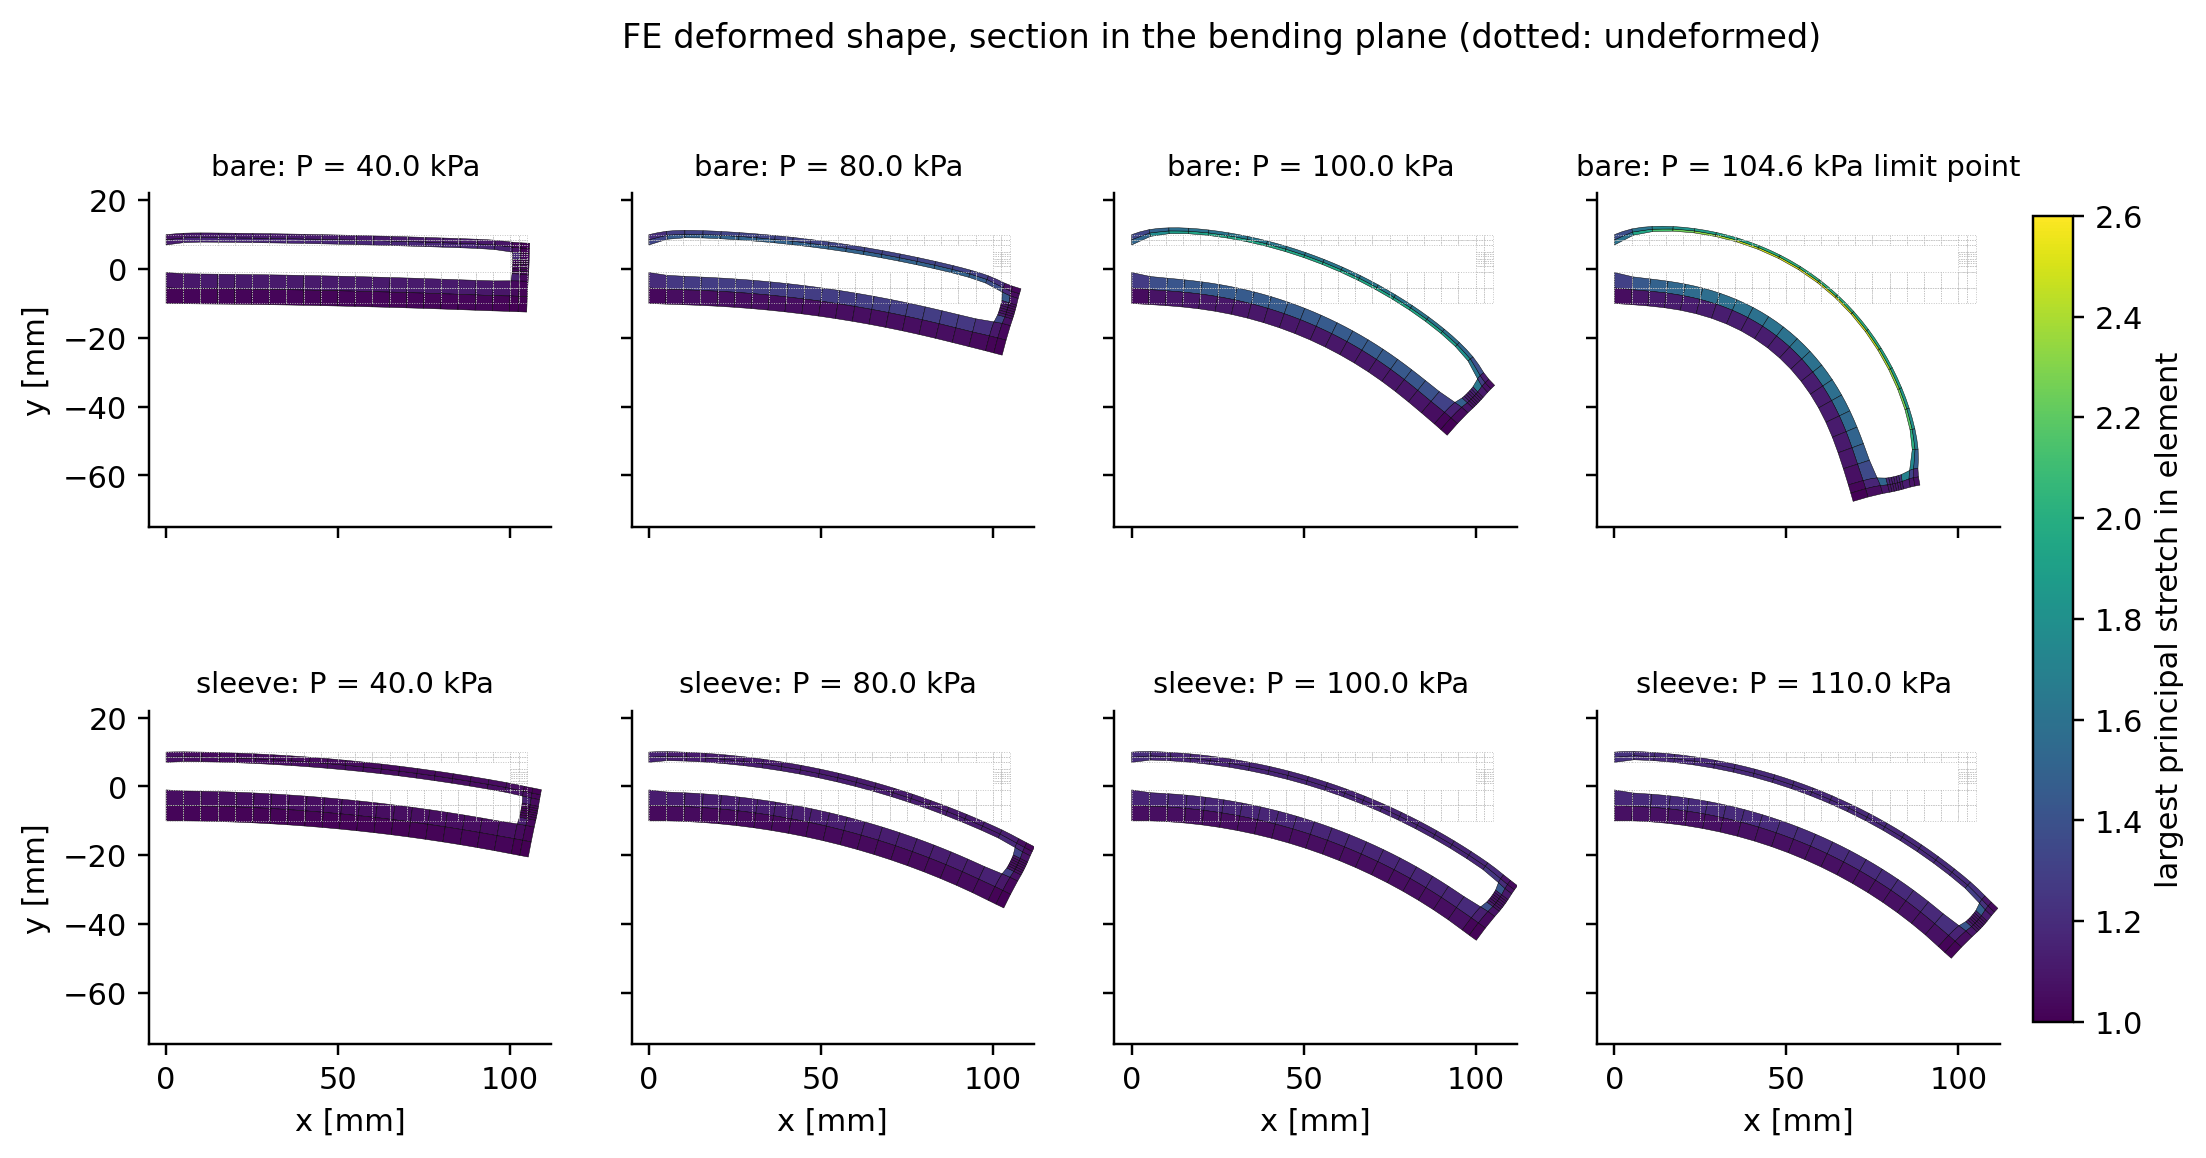
\includegraphics[width=\textwidth]{figures/fe_deformed_sections.png}
\caption{Deformed section in the bending plane, coloured by the largest principal stretch. Top: bare actuator, with the thin wall ballooning near the limit. Bottom: sleeved actuator.}
\label{fig:deformed}
\end{figure}

\begin{enumerate}[nosep]
\item \textbf{Bare actuator.} Below $P/\mu\approx0.2$ the beam model over-predicts by a factor of 4 to 10. The curves cross near $P/\mu=0.43$; that is a coincidence of two different mechanisms, not a validation. The response then steepens without bound: between \SI{100}{kPa} and the limit, \SI{4.6}{kPa} adds \SI{23}{mm} of deflection. At the limit the cavity holds four times its original volume and the thin wall is at a third of its thickness.
\item \textbf{Hoop-reinforced actuator.} The response is smooth and nearly linear, with no limit point up to \SI{110}{kPa}. Eq.~(\ref{eq:theta}) holds within 5\,\% up to $P/E\approx0.03$. At higher pressure the FE angle is larger (by 25\,\% at $P/E=0.1$) because the cavity grows as the actuator lengthens inside a sleeve of fixed circumference, and the thrust grows with it.
\item \textbf{Design consequence.} Reinforce the actuator if a predictable, nearly linear $P\to\delta$ map is wanted (e.g.\ for control). Keep it bare only to study ballooning, and then operate below about 90\,\% of the measured limit pressure.
\end{enumerate}

%======================================================================
\section{Conclusions and next steps}
\begin{enumerate}[nosep]
\item The cross-section properties (eqs.~\ref{eq:A}--\ref{eq:I}) and the eccentric thrust moment (eqs.~\ref{eq:F}--\ref{eq:M}) follow from statics alone and hold for any material law.
\item The Euler--Bernoulli result, eq.~(\ref{eq:theta}), is the correct first-order model for a \emph{hoop-reinforced} actuator and has been confirmed by FE.
\item For a \emph{bare} silicone actuator the first-order bending is zero, by the factor $(1-2\nu)$. What bending remains comes from second-order wall lengthening, $\varepsilon_{\text{axial}}\approx\frac23\varepsilon_{\text{hoop}}^2$, and ends at a ballooning limit $P_{\text{lim}}\approx0.52\,\mu$.
\item Next: fix the real geometry and silicone, measure the Yeoh constants (ASTM D412 dumbbells), choose bare or reinforced, re-run the FE sweep with the measured material, then fabricate and test against it.
\end{enumerate}

%======================================================================
\section*{References}
\addcontentsline{toc}{section}{References}
\small
\begin{enumerate}[label={[\arabic*]},nosep,leftmargin=2em]
\item P.~Polygerinos et al., ``Modeling of soft fiber-reinforced bending actuators,'' \emph{IEEE Transactions on Robotics}, 2015.
\item F.~Connolly, C.~J.~Walsh, K.~Bertoldi, ``Automatic design of fiber-reinforced soft actuators for trajectory matching,'' \emph{PNAS}, 2017.
\item R.~J.~Webster III, B.~A.~Jones, ``Design and kinematic modeling of constant curvature continuum robots: a review,'' \emph{IJRR}, 2010.
\item B.~Gorissen et al., ``Elastic inflatable actuators for soft robotic applications,'' \emph{Advanced Materials}, 2017.
\item A.~D.~Marchese, R.~K.~Katzschmann, D.~Rus, ``A recipe for soft fluidic elastomer robots,'' \emph{Soft Robotics}, 2015.
\item O.~H.~Yeoh, ``Some forms of the strain energy function for rubber,'' \emph{Rubber Chemistry and Technology}, 1993.
\item G.~A.~Holzapfel, \emph{Nonlinear Solid Mechanics}, Wiley, 2000.
\end{enumerate}

\end{document}
